% !TEX root = ../main.tex

% Local Variables:
% TeX-master: "../main"
% End:
% chktex-file 26

%%%%%%%%%%%%%%%%%%%%%%%%%%%%%%% Header %%%%%%%%%%%%%%%%%%%%%%%%%%%%%%%%%%%%%%%%%%%%
\begin{minipage}[l]{0.42\textwidth}
    
\includegraphics[width=1\textwidth]{img/logo-UNAMBA.png}
\end{minipage}
\hfill
\begin{minipage}[c]{0.5\textwidth}
    \begin{flushright}
	\large{\textbf{Unidad \#2}}\\
	\large{Lectures on Física I}\\
	\large{22 de Agosto del 2025. Haquira, Apurimac}\\
        % \large{\textbf{Student:} Huallpa Aimituma Josué David}
    \end{flushright}
\end{minipage}
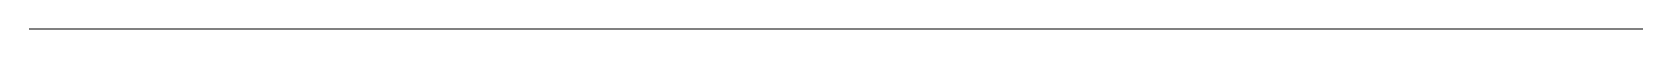
\begin{tikzpicture}
    \draw[gray,thick] (-6.5,0)--(14,0);
\end{tikzpicture}


 %%%%%%%%%%%%%%%%%%%%%%%% INICIO DEL CONTENIDO EN DOS COLUMNAS %%%%%%%%%%%%%%%%%%%%%
  
 \begin{multicols}{2}
   \begin{center}
         \LARGE{\textbf{Capítulo II, III: Vectores -  Estática}}\\	
         \vspace{0.2cm}
         % \Large {Lecturers Esteban Chalbaud \& Daniel Galviz} \\
         % \large{Teaching Assistant: Mauricio Gamonal \& Irvin Martínez}\\
         % \large{PhysicsLatam.com}\\
         % \vspace{0.2cm}
         \large{22 Agosto 2025, 5:59 pm (GMT-4)}\\
         % \vspace{0.2cm}
         \large{— Evaluación Parcial 2 —}
     \end{center}
    %%%%%%%%%%%%%%%%%%%%%%%%%%%%excercise%%%%%%%%%%%%%%%%%%%%%%%%%%%%%%%%%%%%%%%%

    \begin{excercise}[][][]{ex:k28-mod}{(\textbf{4 pts})
        Dados los puntos  $P(-6,\,4,\,-3)$, $Q(4,\,-5,\,2)$ y $R(-2,\,-1,\,7)$:  
        \begin{itemize}
            \item[a)] Construir el vector $\vec{v}=\overrightarrow{PR}$.  
            \item[b)] Encontrar la distancia del punto $Q$ a la recta que pasa por $P$ y es paralela al vector $\vec{v}$.  
            \item[c)] Calcular el ángulo formado por los vectores $\vec{QP}$ y $\vec{v}$.  
            \item[d)] Graficar correctamente los puntos $P$, $Q$, $R$, el vector $\vec{v}$, y la recta solicitada en el ítem (b).  
        \end{itemize}
    }
    \end{excercise}

       %%%%%%%%%%%%%%%%%%%%%%%%%%%%excercise%%%%%%%%%%%%%%%%%%%%%%%%%%%%%%%%%%%%%%%%
    \begin{excercise}[][][a) $R_P= 25\, \mathrm{kgf}  , R_S=21.37\, \mathrm{kgf}$; b)  $R_M=21.37\ \mathrm{kgf}$]{ex:k30}{(\textbf{5 pts})
        Una barra $PQ$ de $5$ m de longitud y $25$ kgf de peso, descanza sobre una superficie lisa formando un ángulo de $70^\circ$ con el piso y se encuentra apoyada por los puntos $S$ y $M$, se conoce que $PS=1$m y $PM=2$m. 
        \begin{figure}[H]
             \centering
             \includegraphics[width=0.8\linewidth]{img/01_physics-i/03_statics/28_ex.png}
         \end{figure} 
         Considerar que todas las superficies son lisas (no hay fuerzas de fricción) y que el peso actua siempre del centro geométrico de la barra. 
        \begin{itemize}
             \item[a)] Calcular las reacciones en los puntos $P$, $S$ y $M$ 
             \item[b)] Resolver el problema usando el método vectorial y escalar para la segunda condición de quilibrio.
         \end{itemize} 
         }
    \end{excercise}
    
    \begin{excercise}[][][$R_A=1143 \ \mathrm{N}$, $R_B=1797\ \mathrm{N}$]{ex:16}{
        (\textbf{4 pts})
         La viga AB es uniforme y tiene una masa de 100 kg. Descansa en sus extremos A y B y soporta las masas como se indica en la Fig. Calcular la reacción en los soportes.         
         \begin{figure}[H]
             \centering
             \includegraphics[width=0.7\linewidth]{img/01_physics-i/03_statics/8.png}
         \end{figure}
         \begin{itemize}
             \item[a)] Calcular la reacción en los soportes. 
             \item[b)] Encontrar la magnitud y posición de la resultante del sistema de fuerzas.
             \item[c)] Calcular el item (a) a traves del método escalar y vectorial.
         \end{itemize}
         }
     \end{excercise}

    %%%%%%%%%%%%%%%%%%%%%%%%%%%%excercise%%%%%%%%%%%%%%%%%%%%%%%%%%%%%%%%%%%%%%%%
     \begin{excercise}[][][$R=25.7\ \mathrm{lbf}$, $y=$]{ex:12}{
         (\textbf{4 pts})
         Encontrar la magnitud y la posición de la resultante de las fuerzas representadas en la Fig.  Cada cuadrado tiene 1 pie de lado.
         \begin{figure}[H]
             \centering
             \includegraphics[width=0.8\linewidth]{img/01_physics-i/03_statics/4.png}
         \end{figure}
         }
     \end{excercise}
    %%%%%%%%%%%%%%%%%%%%%%%%%%%%excercise%%%%%%%%%%%%%%%%%%%%%%%%%%%%%%%%%%%%%%%%
    \begin{excercise}[][][$P=587\ \mathrm{Kgf} $, $R=81.5\ \mathrm{Kgf}$]{ex:30}{
        (\textbf{3 pts})
        Calcular el peso P necesario para mantener el equilibrio en el sistema mostrado en la Fig. En la cual A pesa 100 kgf y Q 10 kgf. El plano y las poleas son lisas. La cuerda AC es horizontal y la cuerda AB es paralela al plano. Calcular también la reacción del plano sobre el peso A.     
         \begin{figure}[H]
             \centering
             \includegraphics[width=0.7\linewidth]{img/01_physics-i/03_statics/19.png}
         \end{figure}
         } 
     \end{excercise}

\end{multicols}
